%
% proposed.tex
%
% Copyright (C) 2023 by Gabriel Mariano Marcelino.
%
% Towards the Conception of GNSS Networks Based on Small Satellites
%
% This work is licensed under the Creative Commons Attribution-ShareAlike 4.0
% International License. To view a copy of this license,
% visit http://creativecommons.org/licenses/by-sa/4.0/.
%

%
% \brief Proposed work slides.
%
% \author Gabriel Mariano Marcelino <gabriel.mm8@gmail.com>
%
% \version 1.0.0
%
% \date 2023/09/09
%

\begin{frame}{Proposed Work}

    Divided into:
    \begin{itemize}
        \item Orbit study
        \vspace{0.1cm}
        \item Communication study
        \vspace{0.1cm}
        \item Required power budget
        \vspace{0.1cm}
        \item Possible technical solutions
        \vspace{0.1cm}
        \item Proposed experiment
    \end{itemize}

\end{frame}

\begin{frame}{Orbit Study}

    \begin{itemize}
        \item Current GNSS networks operate mostly in MEO
        \vspace{0.1cm}
        \item Higher altitudes require more robust components
        \vspace{0.1cm}
        \item Lower altitudes make the design of onboard electronics easier
        \vspace{0.1cm}
        \item To achieve the same coverage as a constellation operating at a higher altitude, lower altitudes require a larger number of satellites in the constellation
        \vspace{0.1cm}
        \item In addition to complexity and the number of satellites, the cost and ease of launching and replacement of the fleet should also be taken into account
        \vspace{0.1cm}
        \item \textbf{Trade-off}: Higher altitudes with fewer but more complex satellites $\times$ Lower altitudes with more but simpler satellites
    \end{itemize}

\end{frame}

%\begin{frame}{Orbit Analysis}
%
%    \begin{figure}[!ht]
%        \begin{center}
%            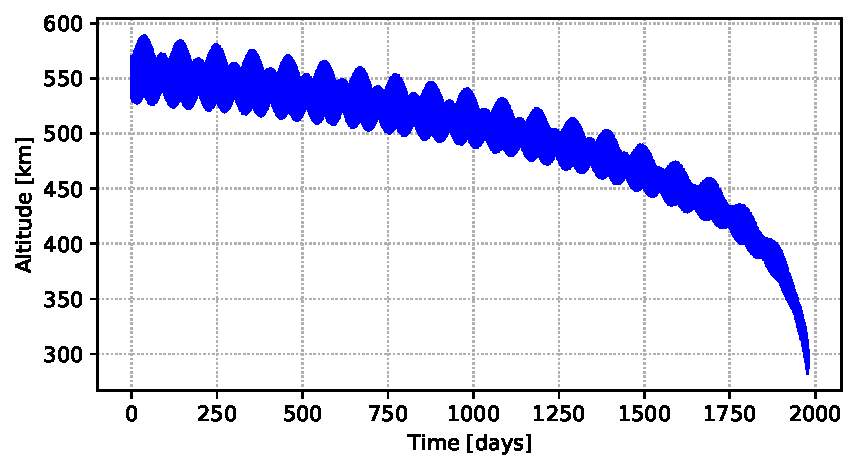
\includegraphics[width=0.8\columnwidth]{figures/lifetime}
%        \end{center}
%    \end{figure}
%
%\end{frame}

\begin{frame}{Communication Study: Link Budget Analysis}

    \begin{itemize}
        \item Conditions:
            \begin{itemize}
                \item \textbf{Altitude}: 550 km
                \vspace{0.1cm}
                \item \textbf{Elevation}: 0$^{\circ}$ (worst case with the satellite at the horizon)
                \vspace{0.1cm}
                \item \textbf{Frequency}: 900 MHz
                \vspace{0.1cm}
                \item \textbf{Transmitter power}: 30 dBm (1 W)
            \end{itemize}
        \item Results:
            \begin{itemize}
                \item \textbf{Free-Space-Path-Loss}: 146.3 $\leq$ FSPL$^{dB}$ $\leq$ 160.2 dB
                \vspace{0.1cm}
                \item \textbf{Power at receiver}: $\geq$ -129.2 dBm
                \vspace{0.1cm}
                \item \textbf{SNR}: $\geq$ 10.4 dB
            \end{itemize}
    \end{itemize}

\end{frame}

\begin{frame}{Power Budget: Subsystems' Consumption}

    \begin{table}[!ht]\scriptsize
        \centering
        \begin{tabular}{lcccc}
            \toprule[1.5pt]
            \textbf{Subsystem} & \textbf{Manufacturer} & \textbf{Model} & \textbf{Consumption [mW]} \\
            \midrule
            OBDH     & GomSpace & NanoMind A3200 & 170 \\
            EPS      & GomSpace & NanoPower P60  & 160 \\
            Battery  & GomSpace & NanoPower BP4  & 50-7000 \\
            TMTC     & GomSpace & NanoCom AX100  & 300-3300 \\
            Antenna  & ISISpace & AntS           & 35-1800 \\
            ADCS     & ISISpace & iMTQ           & 175-1200 \\
            GNSS Transmitter & \multicolumn{2}{c}{Custom model} & 4720 \\
            \bottomrule[1.5pt]
        \end{tabular}
        \label{tab:power-budget-subsystems}
    \end{table}

\end{frame}

\begin{frame}{Power Budget: Mean Power Consumption}

    \begin{table}[!ht]\scriptsize
        \centering
        \begin{tabular}{lcc}
            \toprule[1.5pt]
            \textbf{Subsystem} & \textbf{Duty Cycle [\%]} & \textbf{Power [mW]} \\
            \midrule
            OBDH                  & 100 & 170 \\
            TMTC (RX)             & 95  & 300 \\
            TMTC (TX)             & 5   & 3300 \\
            EPS                   & 100 & 160 \\
            Battery (idle)        & 90  & 50 \\
            Battery (heater full) & 10  & 7000 \\
            ADCS (idle)           & 90  & 175 \\
            ADCS (full actuation) & 10  & 1200 \\
            Antenna (deployment)  & 0   & 1800 \\
            Antenna (deployed)    & 100 & 35 \\
            Payload GNSS          & 100 & 4720 \\
            \cmidrule{2-3}
            Satellite             & \multicolumn{2}{c}{$\cong$ 6526 mW} \\
            \bottomrule[1.5pt]
        \end{tabular}
        \label{tab:power-duty-cycle}
    \end{table}

\end{frame}

\begin{frame}{Power Budget: Input Power}

    \begin{itemize}
        \item Simulated input power for a 6U CubeSat and a solar irradiance of 1367 W/m$^{2}$:
    \end{itemize}

    \begin{figure}[!ht]
        \begin{center}
            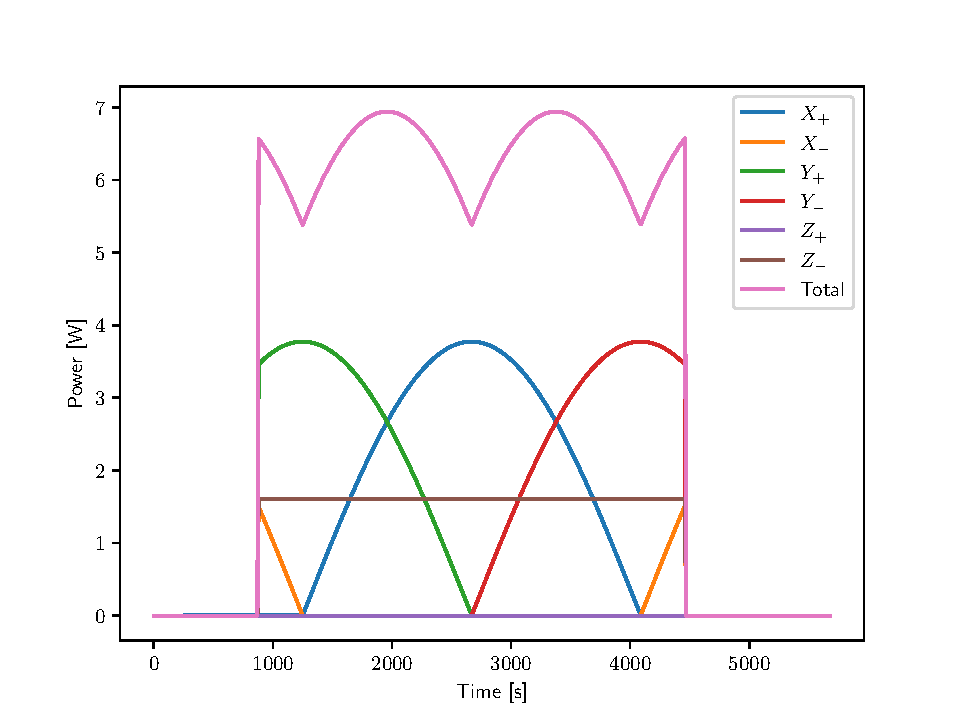
\includegraphics[width=0.7\columnwidth]{figures/sim-input-power-3u}
        \end{center}
    \end{figure}

\end{frame}

\begin{frame}{Power Budget: Preliminary Results}

    \begin{itemize}
        \item For the giving condition, considering a satellite without mechanisms for solar panel deployment, the minimum CubeSat size from the power requirements perspective would be 6U
        \vspace{0.2cm}
        \item Considering the possibility of using mechanisms for panel deployment, the use of a 3U CubeSat would also be possible
    \end{itemize}

\end{frame}

\begin{frame}{Possible Solutions: Clock Reference}

    \begin{columns}[t]
        \begin{column}[t]{0.65\textwidth}
            \begin{itemize}
                \item Quartz oscillator (XO)
                \vspace{0.1cm}
                \item Temperature Compensated Crystal Oscillators (TCXO)
                \vspace{0.1cm}
                \item Oven Controlled Crystall Oscillators (OCXO)
                \vspace{0.1cm}
                \item Rubidium oscillators (RbXO)
                \vspace{0.1cm}
                \item Cesium oscillators
                \vspace{0.1cm}
                \item GPS disciplined oscillators (GPSDO)
            \end{itemize}
        \end{column}
        \begin{column}[t]{0.4\textwidth}
            \begin{figure}[!ht]
                \begin{center}
                    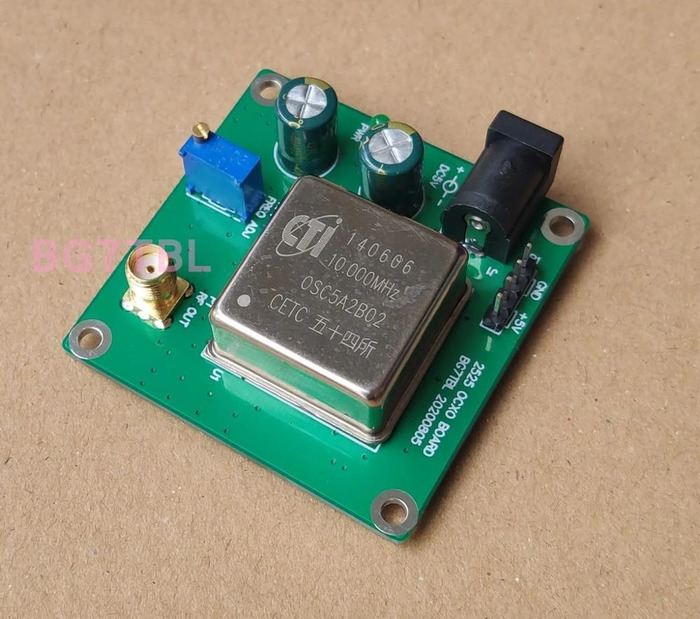
\includegraphics[width=0.8\columnwidth]{figures/ex-ocxo}
                \end{center}
            \end{figure}

            \begin{figure}[!ht]
                \begin{center}
                    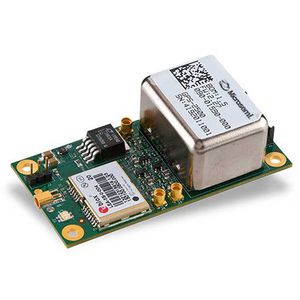
\includegraphics[width=0.8\columnwidth]{figures/gps-2550}
                \end{center}
            \end{figure}
        \end{column}
    \end{columns}

\end{frame}

\begin{frame}{Comparison Between Clock Reference Types}

    \begin{table}[!ht]\tiny
        \centering
        \begin{tabular}{lcccc}
            \toprule[1.5pt]
            \textbf{Oscillator Type} & \textbf{Accuracy} & \textbf{Aging/10 year} & \textbf{Power} & \textbf{Weight} \\
            \midrule
            XO                   & $10^{-5}$ to $10^{-4}$   & 10-20 PPM                                 & 20 $\mu$W  & 20 g \\
            TXCO                 & $10^{-6}$                & 2-5 PPM                                   & 100 $\mu$W & 50 g \\
            MCXO                 & $10^{-8}$ to $10^{-7}$   & 1-3 PPM                                   & 200 $\mu$W & 100 g \\
            OCXO (5 to 10 MHz)   & $10^{-8}$                & $2 \times 10^{-8}$ to $2 \times 10^{-7}$  & \multirow{2}{*}{1-3 W} & \multirow{2}{*}{200-500 g} \\
            OCXO (15 to 100 MHz) & $5 \times 10^{-7}$       & $5 \times 10^{-10}$ to $5 \times 10^{-9}$ &            &  \\
            RbXO                 & $10^{-9}$                & $5 \times 10^{-10}$ to $5 \times 10^{-9}$ & 6-12 W & 1,5-2,5 kg \\
            Cs                   & $10^{-12}$ to $10^{-11}$ & $10^{-12}$ to $10^{-11}$                  & 25-40 W & 10-20 kg \\
            GPS                  & $4 \times 10^{-8}$ to $10^{-11}$ & $10^{-13}$ & 4 W & 340 g \\
            \bottomrule[1.5pt]
        \end{tabular}
        \label{tab:osc-comp}
    \end{table}

\end{frame}

\begin{frame}{Chip Scale Rubidium Oscillator (RbXO)}

    \begin{columns}[t]
        \begin{column}[t]{0.68\textwidth}
            \begin{itemize}
                \item \textbf{Model}: Microchip CSAC-SA-45S
                \vspace{0.2cm}
                \item \textbf{Power consumption}: 120 mW
                \vspace{0.2cm}
                \item \textbf{Volume}: 17 cm$^{3}$
                \vspace{0.2cm}
                \item \textbf{Weight}: 35 g
                \vspace{0.2cm}
                \item \textbf{Accuracy}: $\pm 5 \times 10^{-11}$
                \vspace{0.2cm}
                \item \textbf{Operating temperature}: -10 to 70 $^{\circ}$C
            \end{itemize}
        \end{column}
        \begin{column}[t]{0.5\textwidth}
            \begin{figure}[!ht]
                \begin{center}
                    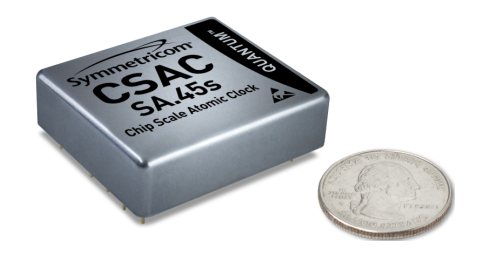
\includegraphics[width=\columnwidth]{figures/microchip-csac}
                \end{center}
            \end{figure}
        \end{column}
    \end{columns}

\end{frame}

\begin{frame}{Possible Solutions: Radio transmitters}

    \begin{itemize}
        \item One solution to overcome the ionospheric delay problem is to use two different frequencies, which will require the use of two radio transmitters
        \vspace{0.2cm}
        \item The use of SDRs is a possible solution for transmitting the signals
    \end{itemize}

\end{frame}

\begin{frame}{Possible Solutions: Antennas}

    \begin{columns}[t]
        \begin{column}[t]{0.7\textwidth}
            \begin{itemize}
                \item Patch antennas are a suitable option for this kind of system, as they are mechanically simpler and suitable for the CubeSat standard size (considering typical frequencies for GNSS systems)
                \vspace{0.2cm}
                \item Depending on the chosen frequency for the system, it is possible that a custom antenna will be required
            \end{itemize}
        \end{column}
        \begin{column}[t]{0.3\textwidth}
            \begin{figure}[!ht]
                \begin{center}
                    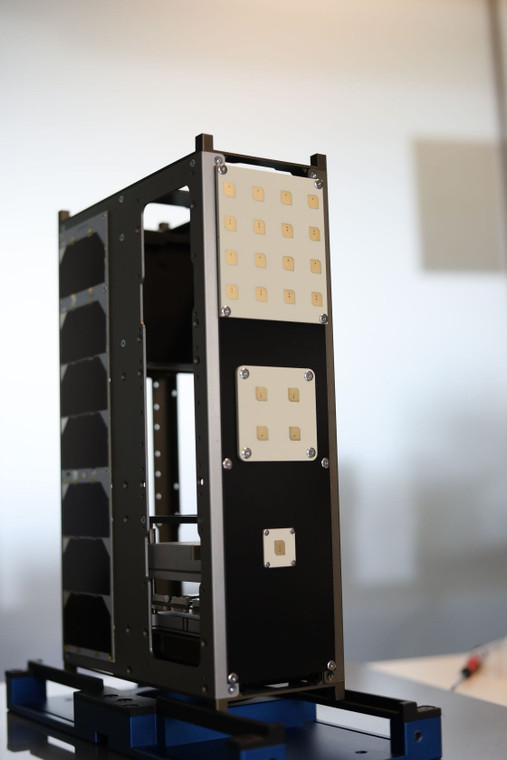
\includegraphics[width=\columnwidth]{figures/x-band-patch-array}
                \end{center}
            \end{figure}
        \end{column}
    \end{columns}

\end{frame}

\begin{frame}{Possible Solutions: Attitude and Orbit Control}

    \begin{itemize}
        \item For the attituce control, magnetic and mechanical solutions cane be considered. As example: magnetorequers and reaction wheels
        \vspace{0.2cm}
        \item Considering a constellation of satellites, to control the position of the objects and to avoid dead zones with no satellite in sign during the operation, a orbit control system is required (ion thruster-based and/or propellant-based thrusters)
    \end{itemize}

\end{frame}

\begin{frame}{Proposed Experiment}

    \begin{itemize}
        \item Development of a payload with an embedded atomic clock and radio transmitters for testing the proposed system
        \vspace{0.5cm}
        \item This payload is intended to be installed on a future CubeSat mission
    \end{itemize}

\end{frame}

\begin{frame}{Proposed Experiment: Block Diagram}

    \begin{figure}[!ht]
        \begin{center}
            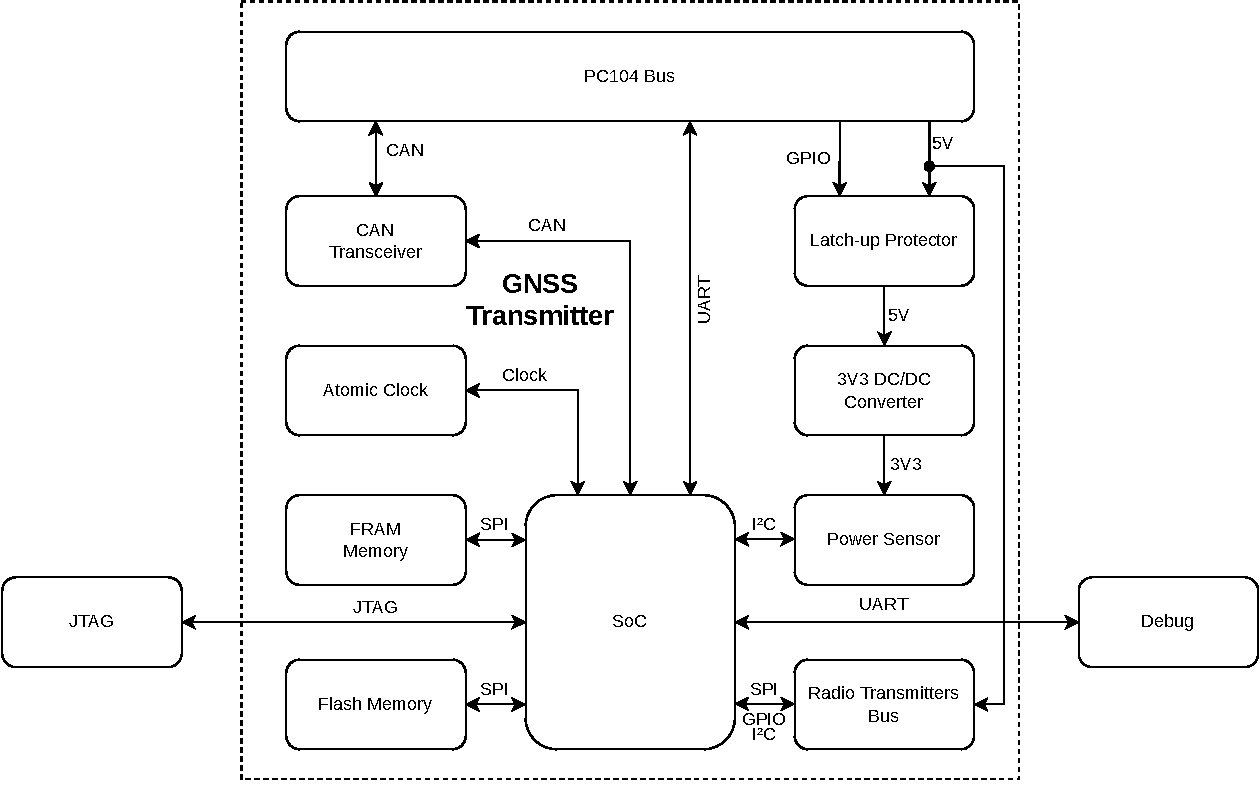
\includegraphics[scale=0.5]{figures/block-diagram}
        \end{center}
    \end{figure}

\end{frame}

\begin{frame}{Proposed Experiment: Block Diagram}

    \begin{figure}[!ht]
        \begin{center}
            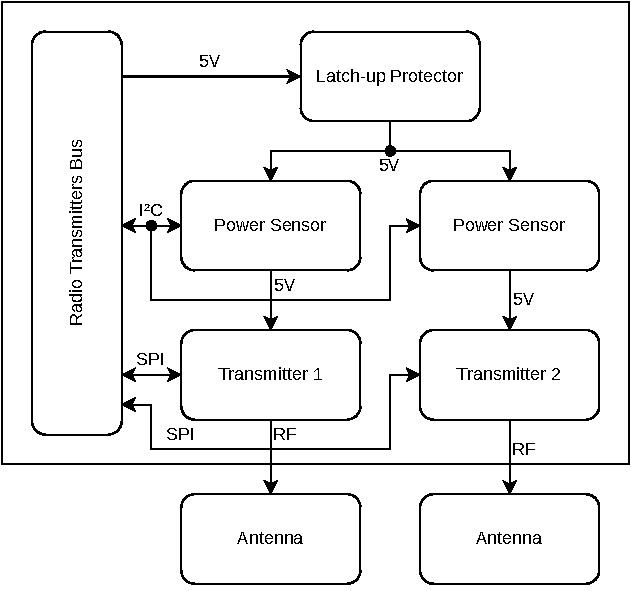
\includegraphics[scale=0.55]{figures/radios-block-diagram}
        \end{center}
    \end{figure}

\end{frame}
